\documentclass{beamer}
\usetheme{default}
\usepackage{import}
\setbeamertemplate{frametitle continuation}[from second] 
\title{S3 performance em HPC}
\author{João Pedro Abreu de Souza}
\begin{document}
\begin{frame}{Analyzing the Performance of the S3 Object Storage API for HPC Workloads}
\end{frame}
\begin{frame}{Organização do artigo}
 \begin{itemize}
     \item introdução
     \item materiais e métodos
     \item resultados
     \item S3Embedded
     \item conclusão
 \end{itemize}   
\end{frame}
\begin{frame}{introdução}
\begin{itemize}
    \item With the increased prevalence of cloud computing and the increased use of the Infrastructure as a Service (IaaS), various APIs are provided to access storage.
    \item The Amazon Simple Storage Service (S3) API is the most widely adopted object storage in the cloud.
\end{itemize}    
\end{frame}
\begin{frame}{introdução - S3}
	\begin{itemize}
		\item 	Um dos primeiros serviços da AWS, lançado em 2006.
		\pause
		\item	Armazenamento de arquivos (objetos), sem noção de hierarquias
		\pause
		\item	Unidade lógica de coleção de objetos é o Bucket
		\pause
		\item	Cada objeto possui um nome, chamado de chave, único no seu bucket.
		\pause
		\item	Um dos serviços mais utilizados para armazenar documentos na AWS, liberando espaço de serviços mais caros como RDS.
	\end{itemize}
\end{frame}
\begin{frame}{introdução - Object Storage API}
	\begin{itemize}
		\item API REST estável (i.e última atualização da API data de 1/3/2006)
		\pause
		\item Capacidade de receber arquivos de até 5TB
		\pause
		\item Controle majoritário via cabeçalhos customizados e parâmetros de consulta na url
		\pause
		\item Poucos endpoints
		\pause
		\item Pelas idiossincrasias da api, sugere-se acessa-la via bibliotecas
		\pause
		\item Tendo se tornado padrão de fato no armazenamento de objetos, múltiplas implementações fora da aws surgiram
		\begin{itemize}
			\item On-premises
				\begin{itemize}
					\item Swift
					\item MinIO
				\end{itemize}
			\item Cloud
				\begin{itemize}
					\item Google
					\item IBM
				\end{itemize}
		\end{itemize}
	\end{itemize}
\end{frame}
\begin{frame}{introdução - contribuições}
\begin{itemize}
    \item The modification of
existing HPC benchmarks to quantify the performance of the S3 API by displaying relevant performance characteristics and providing a deep analysis of the latency of individual operations
    \item the creation of a high-performance I/O library called S3Embedded, which can be used as a drop-in replacement of the commonly used libs3, and which is also compatible and competitive with the HPC I/O protocols, and optimized for use in
distributed environments
\end{itemize}
\end{frame}
\begin{frame}{introdução - sistema sobre teste}
	\begin{itemize}
		\item Supercomputador Mistral alemão
		\item Performance de 2.54 PetaFLOPS (pico de 3.14 PetaFLOPS)
		\item \#33 na lista top500
	\end{itemize}
\end{frame}
\begin{frame}{materiais e metodos}
    \begin{itemize}
        \item We aim to analyze the performance of the S3 interface of different vendors in an
HPC environment to assess the performance potential of the S3 API
    \end{itemize}
\end{frame}
\begin{frame}{materiais e metodos - IO500}
	\begin{itemize}
		\item Estrutura testes em dois setups : easy e hard
		\item Setup easy feito para mostrar o melhor caso do sistema de armazenamento avaliado, com configurações do usuário do benchmark
		\item Setup hard feito para mostrar o pior caso do sistema de armazenamento avaliado, com configurações pré-configuradas.
		\item O artigo utilizou dois benchmarks do IO500, a saber, IOR e MDTest nos dois setups, para colher as metricas
		\begin{itemize}
			\item IOEasy simulating applications with well-optimized I/O patterns.
			\item IOHard simulating applications that utilize segmented input to a shared file.
			\item MDEasy simulating metadata access patterns on small objects.
			\item MDHard accessing small files (3901 bytes) in a shared bucket.
		\end{itemize}
		\end{itemize}
	\end{frame}
 \begin{frame}{materiais e metodos - IO500 - modificações s3}
	For IO500, an optimistic S3 interface backend using the libS3 client library is implemented for IOR in the sense that it stores each fragment as one independent object, and as
	such, it is expected to generate the best performance for many workloads.
	For identifying bottlenecks, it supports two modes:
\begin{itemize}
	\item 	Single bucket mode: created files and directories result in one empty dummy object
	(indicating that a file exists), every read/write access happens with exactly one object
	(file name contains the object name + size/offset tuple); deletion traverses the prefix
	and removes all the objects with the same prefix recursively.
	\item	One bucket per file mode: for each file, a bucket is created. Every read/write access
	happens with exactly one object (object name contains the filename + size/offset
	tuple); deletion removes the bucket with all contained objects.
	
\end{itemize}
	
\end{frame}
\begin{frame}{materiais e metodos - MD-Workbench}
	\begin{itemize}
		\item Possui dois modos
		\begin{itemize}
			\item One bucket, the D datasets are prefixed by the process rank.
			\item One bucket per dataset.
		\end{itemize}
		\item	MD-Workbench casa muito melhor com a API do S3
	\end{itemize}
\end{frame}
\begin{frame}{materiais e metodos - MD-Workbench - modificações s3}
	\begin{itemize}
		\item 	O MD-Workbench funciona com um sistema de plugins, em que o arquivo principal possui um array de vtables com operações de IO
		\item	A adição do suporte ao S3 foi apenas questão de adicionar um novo plugin, implementando as chamadas de IO como chamadas a libs3 e adicionar esse plugin ao array supracitado
	\end{itemize}

\end{frame}

\begin{frame}{materiais e metodos - minIO}
	\begin{itemize}
		\item 	MinIO is a high-performance, S3 compatible object store. It is built for
		large scale AI/ML, data lake and database workloads. It is software-defined
		and runs on any cloud or on-premises infrastructure.
		\item	Pode utilizar multiplos backends para prover essa interface. O lustre é utilizado como backend do minIO a fim de rodar os testes sob uma mesma interface mas com uma baseline de um sistema de arquivos tipico.
	\end{itemize}
\end{frame}
\begin{frame}{materiais e metodos - minIO - modos}
	\begin{itemize}
		\item gateway (gw)
		\begin{itemize}
			\item in this mode, any a S3 request is converted to POSIX requests for the shared file system.
		\end{itemize}
		\item Standalone (sa)
		\begin{itemize}
			\item runs one MinIO server on one node with a single storage device. We
			test configurations from tmpfs (in-memory fs/shm) and the local ext4 file system
		\end{itemize}
		\item Distributed servers (srv)
		\begin{itemize}
			\item runs on multiple nodes, object data and parity are striped
			across all disks in all nodes. The data are protected using object-level erasure coding
			and bitrot. Objects are accessible from any MinIO server node. In our setup, each
			server uses the local ext4 file system
		\end{itemize}
	\end{itemize}
\end{frame}
\begin{frame}{materiais e metodos - minIO - modos - distributed servers}
    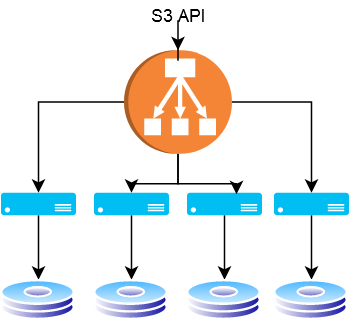
\includegraphics[width=0.6\paperwidth]{presentation/5.png}
\end{frame}
\begin{frame}{materiais e metodos - minIO - modos - gateway}
    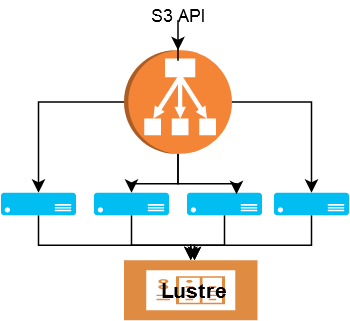
\includegraphics[width=0.6\paperwidth]{presentation/6.png}
\end{frame}
\begin{frame}{resultados - Analyzing the Performance ...}
	\begin{itemize}
		\item Para se analisar algo, precisamos de métricas e testes padronizados
		\pause
		\item Benchmarks
		\begin{itemize}
			\item IO500
			\item MD-Workbench
		\end{itemize}
	\end{itemize}
´\end{frame}

\begin{frame}{resultados - IO500 - metricas}
	Metricas avaliadas : 
		\begin{itemize}
			\item ior-easy-write
			\item mdtest-easy-write
			\item ior-hard-write
			\item mdtest-hard-write
			\item ior-easy-read
			\item mdtest-easy-stat
			\item ior-hard-read
			\item mdtest-hard-stat
			\item mdtest-easy-delete
			\item mdtest-hard-read
			\item mdtest-hard-delete
		\end{itemize}

\end{frame}


\begin{frame}{resultados - MD-Workbench - metricas}
	\begin{itemize}
		\item rate
		\item throughput
	\end{itemize}
\end{frame}

\begin{frame}{resultados - fase 1 - minIO - single client}
	\begin{itemize}
		\item The first tests are performed using IOR directly
		\item the standalone mode shows the best performance
		\item Gateway mode is effective for reads,
		but slow for writes
		\item Write performance is 1/3rd of the read performance
		\item Adding a load balancer has minimal
		influences on throughput in this setting, except when activating the caching mechanism,
		which has a tremendous impact on the read throughput.
		\item Compared to the
		Infiniband network throughput (about 6 GiB/s), only 7.5\% and 2.5\% of this performance
		can be obtained for read and write, respectively.
	\end{itemize}
\end{frame}
\begin{frame}{resultados - fase 1 - minIO - single client}
    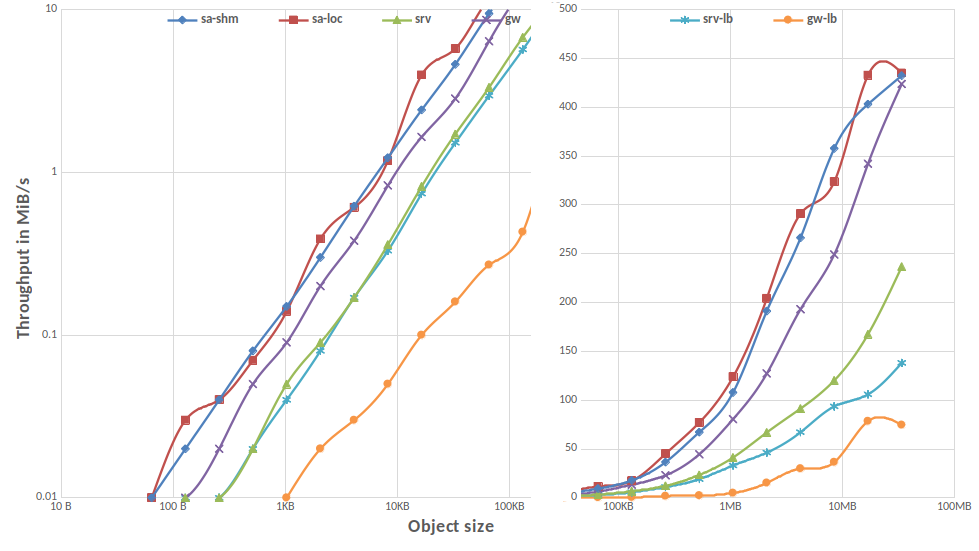
\includegraphics[width=0.9\paperwidth]{presentation/7.png}
\end{frame}
\begin{frame}{resultados - fase 1 - minIO - single client}
    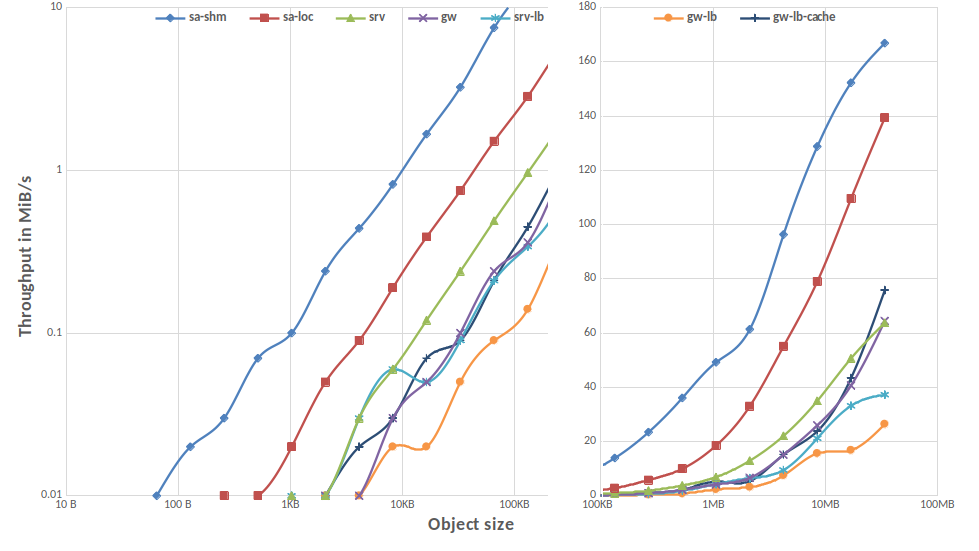
\includegraphics[width=0.9\paperwidth]{presentation/8.png}
\end{frame}
\begin{frame}{resultados - fase 1 - minIO - parallel IO}
	\begin{itemize}
		\item Assuming an ideal scenario, we
		start MinIO in standalone mode with RAM as backend (sa-shm) on one node.
		\item when increasing the number of tasks per node, we achieve the best
		throughput (about 6000 MiB/s).
		\item The performance per client node is 1.5 GiB/s
		\item For the
		single server, it is close to the available network bandwidth
	\end{itemize}
\end{frame}
\begin{frame}{resultados - fase 1 - minIO - parallel IO}
    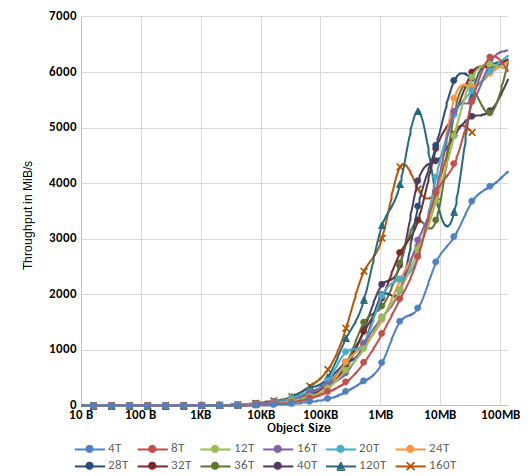
\includegraphics[width=0.7\paperwidth]{presentation/9.png}
\end{frame}
\begin{frame}{resultados - fase 1 - minIO - parallel IO}
    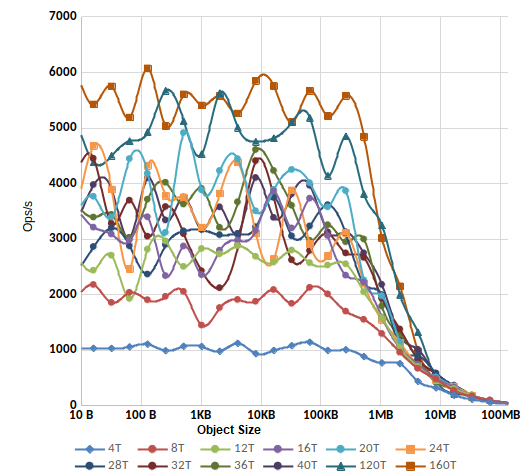
\includegraphics[width=0.7\paperwidth]{presentation/10.png}
\end{frame}
\begin{frame}{resultados - fase 2 - Tests against S3 Compatible Systems}
	\begin{itemize}
		\item The Benchmarks are performed on Mistral using IO500 and MD-Workbench.
		\item Tests are conducted against the OpenStack Swift system already available in DKRZ
		\item Swift version 2.19.2 is used, and the S3 interface is implemented using Swift3 version 1.12.1
		\item the tests were only conducted using MD-Workbench.
		\item o motivo dos testes usarem apenas o MD-Workbench é por uma incompatibilidade de assinaturas nas versões da libse.
		\item On
		four client nodes and with 20 PPN, a rate of 269.5 IOPs and a 0.5 MiB/s throughput are
		observed during the benchmark phase with MD-Workbench.
		\item MD-Workbench reports not only the throughput, but also the latency statistics for
		each I/O operation.
		\item A latencia observada com o swift era menos previsivel do que com o Lustre, levando a conclusão que os processos por trás da implementação do s3 eram a principal origem da latência.
	\end{itemize}
\end{frame}
\begin{frame}{resultados - fase 2 - Tests against S3 Compatible Systems}
    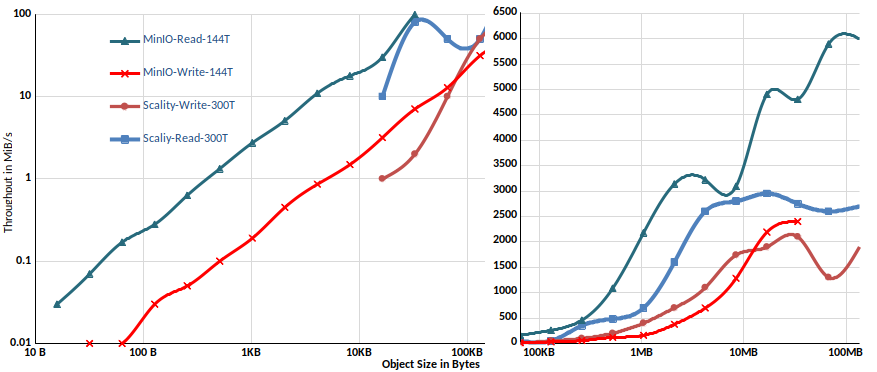
\includegraphics[width=0.9\paperwidth]{presentation/14.png}
\end{frame}
\begin{frame}{resultados - fase 3 - S3Embedded}
	\begin{itemize}
		\item Por conta dos problemas de escalabilidade reportados na fase 2, foi criada uma biblioteca, S3Embedded, baseada na libs3
		\item partes da libs3 foram substituidas, a fim de investigar se aquela parte removida era a causadora da latência
		\item a biblioteca é compativel a nivel de código e binario com a libs3, permitindo que aplicações linkadas dinamicamente com a libs3 possam usar a libEmbedded ao invés.
		\item a biblioteca contém sub-bibliotecas
		\begin{itemize}
			\item libS3e.so: This is an embedded library wrapper that converts libs3 calls to POSIX calls
			inside the application address space.
			\item ibS3r.so: This library converts the libs3 calls via a binary conversion to TCP calls to a local
			libS3-gw application that then executes these POSIX calls, bypassing the HTTP protocol.
			\item The results delivered by S3Embedded are very close to the ones obtained for the
			Lustre direct access,mainly for files larger than 32 MB
			\item Com mais nós, a biblioteca S3Embedded melhora a performance em relação ao lustre, porém um gap de 10x existe
		\end{itemize}
	\end{itemize}
\end{frame}
\begin{frame}{Conclusão}
	\begin{itemize}
		\item Bibliotecas s3 não estão prontas para hpc
		\item Com o IO-500 aumentado, a comunidade pode observar o s3
		\item integrações entre S3 e sistemas de arquivos permitiriam que clientes s3 acessassem IO de HPC
	\end{itemize}
\end{frame}
\begin{frame}{Adendo}
    fsx - lustre
\end{frame}
\end{document}
